\documentclass[parskip, 12pt, DIV=16, openany]{scrartcl}

\usepackage{german}
\usepackage[utf8]{inputenc}
\usepackage{amsmath}
\usepackage{enumerate}
\usepackage{hyperref}
\usepackage{graphicx}
\usepackage[german]{cleveref}
\usepackage{booktabs}
\usepackage{pdfpages}
\usepackage{afterpage}
\usepackage{float}
\usepackage{siunitx}
%\usepackage[per-mode=fraction, exponent-product=\cdot, output-decimal-marker={,}, uncertainty-mode=separate]{siunitx}
\usepackage[per-mode=fraction, exponent-product=\cdot, output-decimal-marker={,}]{siunitx}

%\usepackage{txfonts}
\usepackage{tikz}

%\usepackage[T1]{fontenc}
%\usepackage{lmodern}

\DeclareUnicodeCharacter{0394}{\ensuremath{\Delta}}

\newcommand{\Z}{\mathbb Z}

%\renewcommand{\thefootnote}{\fnsymbol{footnote}}
\renewcommand{\thefootnote}{\textit\arabic{footnote}}


\newcommand{\DefVal}[2]{%
  \expandafter\newcommand\csname val-#1\endcsname{#2}%
}
\newcommand{\Val}[1]{\csname val-#1\endcsname}
\DefVal{_}{0.7021125760141528}
\DefVal{c1}{12.211599818576055}
\DefVal{dc1}{0.04105725358249311}
\DefVal{X2_1}{0.3882876282488006}
\DefVal{dof_1}{18}
\DefVal{R1}{81.88935232538647}
\DefVal{dR1}{0.2753244418487307}
\DefVal{index}{10}
\DefVal{a2q}{16.185711504480224}
\DefVal{b2q}{-0.08482659918456946}
\DefVal{da2q}{0.06734309521650214}
\DefVal{db2q}{0.0011768583504398933}
\DefVal{X2_2q}{3155.733607790688}
\DefVal{dof_2q}{24}
\DefVal{a2a}{6.128593619547221}
\DefVal{b2a}{22.036837779574704}
\DefVal{da2a}{0.07659683834498186}
\DefVal{db2a}{0.24332252384572234}
\DefVal{X2_2a}{148.82713602429988}
\DefVal{dof_2a}{24}
\DefVal{R1_lit}{82.5}
\DefVal{dR1_lit}{0.8250000000000001}
\DefVal{t}{0.7021125760141528}
\DefVal{_20}{0.7021125760141528}

\newcommand{\SIp}[3]{\SI[round-mode=places,round-precision=#1]{\Val{#2}}{#3}}
\newcommand{\SIu}[3]{\SI[round-mode=uncertainty,round-precision=2]{\Val{#1}\pm\Val{#2}}{#3}}

\begin{document}
\begin{center}

\vspace{2cm}

\large
Universität Freiburg \\
Physiklabor für Anfänger*innen Teil 2\\
Ferienpraktikum im WS 2022/23

\vspace{2cm}
\vspace{2cm}
{\sectfont
 \Huge Versuch 45\\Strom-Spannungs-Kennlinien\par
}
\vspace{2cm}

{\Large
Müller, André\\
Kopp, Manuel\\
Breitner, Joachim\\
(Gruppe 121)\\
}

\end{center}
\vspace{2cm}
\vspace{2cm}
\vspace{2cm}
\vspace{2cm}

{\large
Durchführung: 23. Februar 2023\\
Protokollerstellung: \today\\
Assistent: Steffen Ludwig
}

\pagebreak
\section{Ziel des Versuchs}

Wir messen Strom-Spannungs-Kennlinien für verschiedene zweipolige elektrische Bauteile.


\section{Versuchsdurchführung}

% ref tabelle per \cref{tab1}
Für die Messung der Strom-Spannungs-Kennlinien haben wir uns bei allen Bauteilen für die spannungsrichtige Schaltung entschieden (siehe \cref{fig:schaltungen}). Der Grund dafür ist der geringe Widerstand bei allen Bauteilen ausgenommen der LED bei Spannungen unter \SI{1,8}{\V}. Die Kennlinen haben wir bei allen Bauteilen für positive und negative Spannungen gemessen. Zur Messung von Strom und Spannung verwendeten wir die Digitalmultimeter Uni-T UT51 und Pierron UT51, die laut Versuchsbeschreibung baugleich sind.

Im ersten Versuchsteil haben den Strom $I$ für verschiedene Spannungen $U$ an einem technischen Widerstand gemessen. Den Messbereich der Multimeter haben wir für Spannung auf \SI{2}{\V} und für Strom auf \SI{20}{\mA} eingestellt, da wir nur bei geringer Spannung messen wollten, um ein Erwärmen des Widerstands bei höherer Leistung zu vermeiden. 

Der zweite Versuchsteil unterscheidet sich vom ersten dadurch, dass wir statt eines Widerstands, eine Glühlampe in den Schaltkreis eingesetzt haben. Den Messbereich haben wir auf \SI{20}{\V} und \SI{200}{\mA} eingestellt, da wir in diesem Messbereich dem ganzen Spannungsbereich des Netzgeräts verwenden können.

Im dritten Versuchsteil haben wir die Kennline einer LED vermessen. Um den Stromfluss durch die LED zu begrenzen, haben wir einen Widerstand der Größe \SI{216(2)}{\ohm} (gemessen mit Uni-T UT51) vor die LED geschaltet. Die Spannung haben wir direkt an der LED gemessen, um Fehler durch einen nicht konstanten Widerstand auszuschließen und den Stromfluss durch das Voltmeter zu verringern. Den Messbereich haben wir hier mehrfach geändert, da der Strom mit zunehmender Spannung expotentiell anwächst. Hier haben wir für alle Messungen den kleinstmöglichen Messbereich verwendet. Bei der Messung des Stroms für negative Spannungen haben wir immer \SI{0}{\A} erhalten.

Im vierten Versuchteil haben wir ein unbekanntes Bauteil erhalten. Hier haben wir sowohl die Kennlinie gemessen, als auch das Bauteil auf weitere Eigenschaften untersucht. Auch hier haben wir uns immer für den kleinstmöglichen Messbereich entschieden. Die Messwerte und die daraus errechneten Widerstände $R$ zu den verschiedenen Bauteilen sind in \cref{tab1},\cref{tab2},\cref{tab3} und \cref{tab4} aufgelistet.
\begin{figure}
\centering
\includegraphics[page=2,trim=6cm 5.5cm 6cm 19.5cm,clip]{Versuch 45.pdf}
\caption{verwendeter Schaltungsaufbau (Schaubild aus der Versuchsbeschreibung)}\label{fig:schaltungen}
\end{figure}


\begin{table}
\begin{center}

\begingroup
\sisetup{round-mode=uncertainty,round-precision=2}
\begin{tabular}{SSS}
\toprule
{$U$ (\unit{\V})} & {$I$ (\unit{\mA})} & {$R$ (\unit{\ohm})} \\
\midrule
0.085\pm0.001425 & 1.03\pm0.01645 & 82.5242718446602\pm1.9107963173389984  \\
0.215\pm0.002075 & 2.62\pm0.0403 & 82.06106870229007\pm1.4901282445500277  \\
0.352\pm0.00276 & 4.29\pm0.06535 & 82.05128205128206\pm1.4057547050767423  \\
0.424\pm0.00312 & 5.18\pm0.07869999999999999 & 81.85328185328186\pm1.3817846378985987  \\
0.502\pm0.00351 & 6.13\pm0.09294999999999999 & 81.89233278955955\pm1.3674035526704096  \\
0.602\pm0.00401 & 7.36\pm0.1114 & 81.79347826086956\pm1.3526010073176424  \\
0.703\pm0.004515 & 8.59\pm0.12985 & 81.83934807916181\pm1.3441453878077414  \\
0.859\pm0.005295 & 10.5\pm0.1585 & 81.80952380952381\pm1.3339290309657137  \\
0.968\pm0.00584 & 11.83\pm0.17845 & 81.82586644125107\pm1.3293640343097142  \\
1.06\pm0.0063 & 12.96\pm0.19540000000000002 & 81.79012345679013\pm1.325516709988082  \\
-0.156\pm0.00022000000000000003 & -1.9\pm0.027499999999999997 & 82.10526315789474\pm1.1939933511625174  \\
-0.405\pm0.0010250000000000003 & -4.96\pm0.07339999999999999 & 81.65322580645163\pm1.2258799080636815  \\
-0.553\pm0.001765 & -6.76\pm0.10039999999999999 & 81.80473372781066\pm1.2427074615075924  \\
-0.604\pm0.00202 & -7.38\pm0.10969999999999999 & 81.84281842818427\pm1.2469637361303585  \\
-0.704\pm0.0025199999999999997 & -8.6\pm0.128 & 81.86046511627906\pm1.2531291720770055  \\
-0.747\pm0.002735 & -9.12\pm0.13579999999999998 & 81.90789473684211\pm1.2559655039773003  \\
-0.793\pm0.0029650000000000006 & -9.69\pm0.14434999999999998 & 81.83694530443756\pm1.2569220811332358  \\
-0.876\pm0.00338 & -10.71\pm0.15965000000000001 & 81.79271708683473\pm1.2594357869337793  \\
-0.94\pm0.0037 & -11.49\pm0.17135 & 81.81026979982593\pm1.2618157927322506  \\
-1.551\pm0.006755 & -18.96\pm0.2834 & 81.80379746835442\pm1.2735901491512711  \\

\bottomrule
\end{tabular}
\endgroup

\end{center}
\caption{technischer Widerstand}
\label{tab1}
\end{table}


\begin{table}
\begin{center}

\begingroup
\sisetup{round-mode=uncertainty,round-precision=2}
\begin{tabular}{SSS}
\toprule
{$U$ (\unit{\V})} & {$I$ (\unit{\mA})} & {$R$ (\unit{\ohm})} \\
\midrule
0.47\pm0.01235 & 16.4\pm0.346 & 28.658536585365855\pm0.9657401960053867  \\
0.95\pm0.01475 & 23.3\pm0.4495 & 40.7725321888412\pm1.00967953484316  \\
1.22\pm0.0161 & 26.8\pm0.502 & 45.52238805970149\pm1.0430655095557169  \\
1.54\pm0.0177 & 30.7\pm0.5605 & 50.1628664495114\pm1.0822058651837434  \\
1.84\pm0.019200000000000002 & 33.9\pm0.6084999999999999 & 54.277286135693224\pm1.126932789788907  \\
2.05\pm0.020249999999999997 & 36.0\pm0.64 & 56.944444444444436\pm1.1581234924717514  \\
2.47\pm0.022350000000000002 & 40.2\pm0.703 & 61.44278606965174\pm1.2098015700314673  \\
2.97\pm0.024850000000000004 & 44.8\pm0.7719999999999999 & 66.29464285714288\pm1.2699421802701198  \\
3.82\pm0.0291 & 52.4\pm0.8859999999999999 & 72.90076335877862\pm1.3519598991210533  \\
4.44\pm0.0322 & 57.2\pm0.958 & 77.62237762237763\pm1.4166862231362554  \\
5.11\pm0.035550000000000005 & 62.3\pm1.0345 & 82.02247191011237\pm1.47669990498443  \\
9.84\pm0.0592 & 92.2\pm1.483 & 106.72451193058568\pm1.832773122203632  \\
6.23\pm0.041150000000000006 & 70.0\pm1.1500000000000001 & 89.00000000000001\pm1.5758926851477044  \\
6.96\pm0.0448 & 74.9\pm1.2235 & 92.92389853137516\pm1.6315173919886545  \\
7.92\pm0.049600000000000005 & 80.9\pm1.3135000000000001 & 97.89864029666253\pm1.7036367240548855  \\
9.05\pm0.05525000000000001 & 87.7\pm1.4155 & 103.19270239452679\pm1.7807197324259318  \\
-1.07\pm0.00465 & -24.6\pm0.269 & 43.49593495934959\pm0.5118110774054557  \\
-2.04\pm0.00020000000000000052 & -35.9\pm0.4385 & 56.82451253481894\pm0.69410449528584  \\
-3.16\pm0.005800000000000001 & -46.5\pm0.5975 & 67.95698924731184\pm0.8820742185078392  \\
-4.08\pm0.010400000000000001 & -54.2\pm0.7130000000000001 & 75.27675276752767\pm1.008683321126557  \\
-4.97\pm0.01485 & -61.1\pm0.8165 & 81.34206219312603\pm1.1138414676404944  \\
-6.0\pm0.019999999999999997 & -68.5\pm0.9274999999999999 & 87.59124087591242\pm1.2214084709417883  \\
-7.08\pm0.0254 & -75.5\pm1.0325 & 93.77483443708608\pm1.3258112556801032  \\
-7.97\pm0.029849999999999995 & -81.4\pm1.121 & 97.91154791154791\pm1.3973642077298354  \\
-8.97\pm0.03485 & -87.2\pm1.208 & 102.86697247706422\pm1.4800195390254645  \\
-9.84\pm0.0392 & -92.3\pm1.2844999999999998 & 106.60888407367281\pm1.5432212503806522  \\

\bottomrule
\end{tabular}
\endgroup

\end{center}
\caption{Glühlampe}
\label{tab2}
\end{table}


\begin{table}
\begin{center}
\begin{tabular}{SSSSSS}
\toprule
{$\varrho$ ($\mathrm{\mu\Omega m}$)} & {$|\frac{\partial \varrho}{\partial U}|\Delta U$} & {$|\frac{\partial \varrho}{\partial I}|\Delta I$} & {$|\frac{\partial \varrho}{\partial l}|\Delta l$} & {$|\frac{\partial \varrho}{\partial d}|\Delta d$} & {$\Delta \varrho$} \\
\midrule
0.1426 & 0.0013 & 0.0029 & 0.0020 & 0.0114 & 0.0120 \\
\bottomrule
\end{tabular}

\end{center}
\caption{LED}
\label{tab3}
\end{table}
 

\begin{table}
\begin{center}

\begingroup
\sisetup{round-mode=uncertainty,round-precision=2}
\begin{tabular}{SSS}
\toprule
{$U$ (\unit{\V})} & {$I$ (\unit{\mA})} & {$R$ (\unit{\ohm})} \\
\midrule
0.018\pm0.00019 & 5.88\pm0.010144 & 3.061224489795918\pm0.032741647749391006  \\
0.0329\pm0.0002645 & 10.74\pm0.0102632 & 3.063314711359404\pm0.02480092612694295  \\
0.0552\pm0.000376 & 18.05\pm0.0104416 & 3.0581717451523547\pm0.020906011214213597  \\
0.281\pm0.002405 & 90.1\pm0.104215 & 3.1187569367369594\pm0.026935215957173637  \\
0.316\pm0.00258 & 100.8\pm0.10474 & 3.134920634920635\pm0.025801690529850704  \\
0.392\pm0.00296 & 123.4\pm0.10588 & 3.1766612641815235\pm0.024141395067797108  \\
0.491\pm0.003455 & 150.0\pm0.107365 & 3.2733333333333334\pm0.023152188359311515  \\
0.57\pm0.0038499999999999997 & 167.5\pm0.10855000000000001 & 3.4029850746268653\pm0.02309062946423602  \\
0.658\pm0.00429 & 185.0\pm0.10987000000000001 & 3.556756756756757\pm0.02328519763826719  \\
0.735\pm0.004675 & 193.4\pm0.11102500000000001 & 3.800413650465357\pm0.024270953802188196  \\
0.771\pm0.004855 & 195.9\pm0.11156500000000001 & 3.9356814701378253\pm0.024884200463898547  \\

\bottomrule
\end{tabular}
\endgroup

\end{center}
\caption{unbekanntes Bauteil}
\label{tab4}
\end{table}

\section{Auswertung}


\subsection{Fehleranalyse und -beiträge}

Die Fehler bei den Messungen ergeben sich aus den Unsicherheiten der Digitalmultimeter.
Mit der Gauß'schen Fehlerfortpflanzung erhält man die Unsicherheit für $R$. Des weiteren erhalten wir durch die gewählte Schaltung einen Fehler bei der Messung des Stroms. Das Amperemeter misst den Gesamtstrom $I_{\rm{ges}}$ durch das Bauteil und das Voltmeter (Innenwiderstand \SI{10}{M\ohm}), was aufgrund der Gleichung

\[
I_{\rm{ges}}= I_1\bigg(1+\frac{R_1}{R_2}\bigg)
\]

dafür sorgt, dass $I_1$ insbesondere bei Bauteilen mit größerem Widerstand signifikant von $I_{\rm{ges}}$ abweicht.
Dies ist bei uns vor allem für niedrigen Spannungen an der LED relevant, da der Widerstand hier verhältnismäßig groß wird.
Die prozentuale Abweichung von $I_1$ erhält man leicht durch das Verhältnis der Widerstände von Bauteil und Voltmeter.
\[
\frac{I_{\rm{ges}}-I_1}{I_1}= \frac{R_1}{R_2}
\]

\subsection{Strom-Spannungs-Kennlinien}

Wir plotten die gemessenen Ströme über die verschieden Spannungen. Bei dem technischen Widerstand erwarten wir einen linearen Zusammenhang von $I$ und $U$. Dies überprüfen wir mittels linearer Regression. Um zu überprüfen ob die Regressionsgerade mit unseren Messdaten übereinstimmt plotten wir zudem noch die $I$-Residuen (siehe \cref{fig1}). Aus dem Residuendiagramm ist deutlich zu erkennen, dass die Messungen mit unserer erwarteten Abhängigkeit übereinstimmen.
Für die Glühlampe überprüfen wir die Zusammenhänge $I = aU + bU^3$ und $I = aU + b arctan(U)$ (siehe \cref{fig2}). Hier scheint die arctan-Funktion auf den ersten Blick sehr gut zur Kennline zu passen. Im Residuendiagramm sieht man dann aber insbesondere für kleine Spannungen deutlich, dass die Messwerte außerhalb des $\SI{68}{\percent}$ Konfidenzbands liegen. Für die $x^3$-Funktion liegen die Werte für große Spannungen sehr gut innerhalb des Konfidenzbands, weichen für kleine Spannungen aber ähnlich stark ab.
Die Kennlinie der LED (siehe \cref{fig3}) ähnelt stark einer Exponentialfunktion.
Bei dem unbekannten Bauteil haben wir eine Kennlinie erhalten, die bei geringer Spannung noch sehr linear verläuft und gegen oben hin stark abflacht (siehe \cref{fig4}).


\begin{figure}
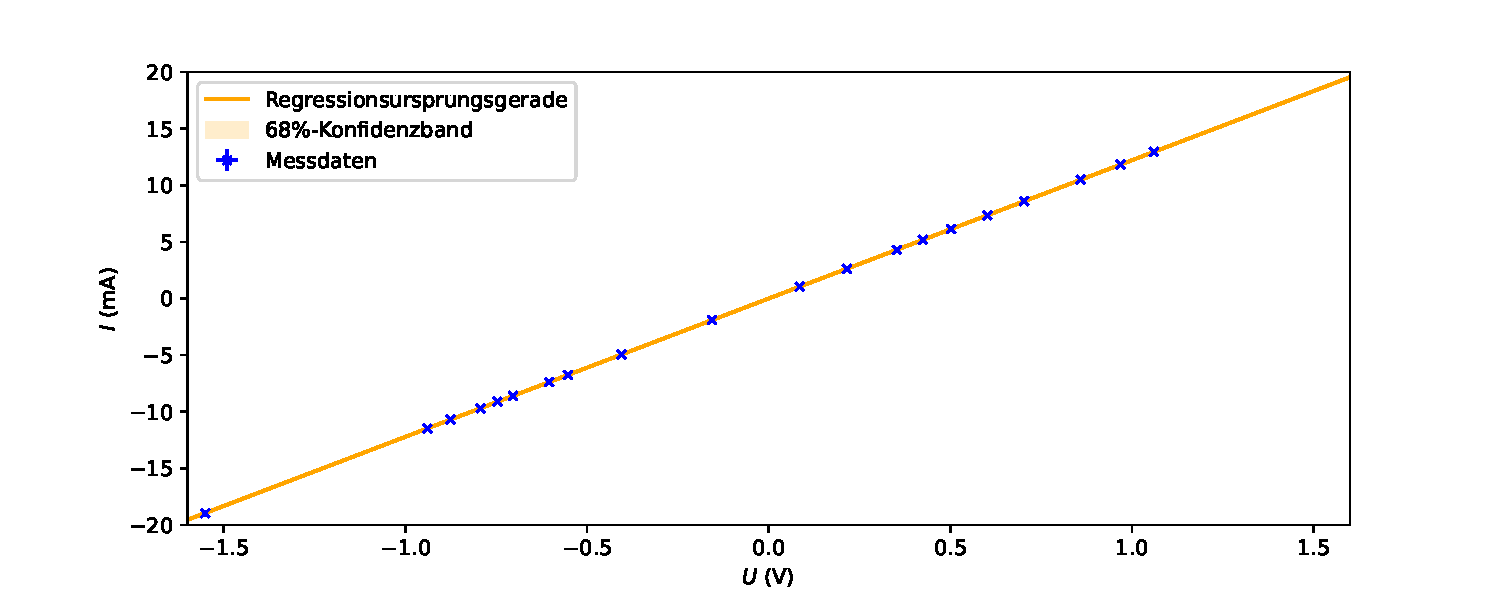
\includegraphics[width=\linewidth]{plot1}%
\vspace*{-1.28cm}\\ % ugly hack
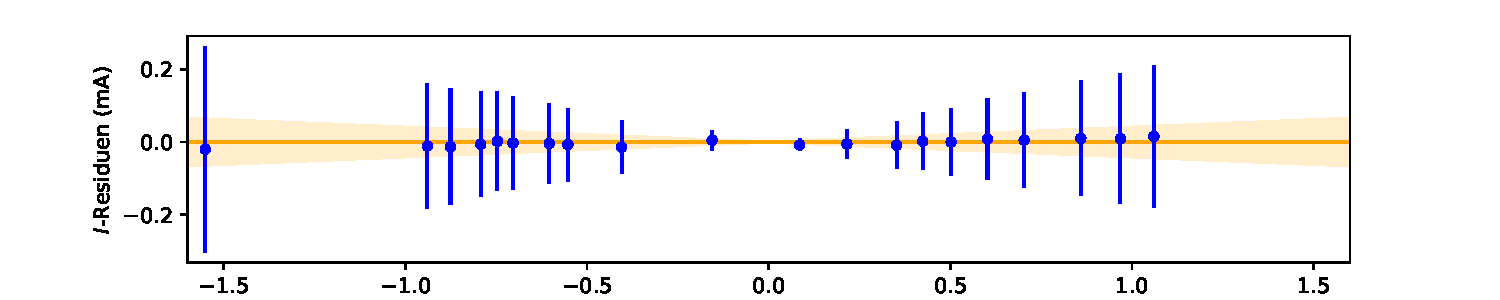
\includegraphics[width=\linewidth]{plot1residuen}
\caption{Kennlinie des technischen Widerstands (oben) Residuendiagramm (unten)}\label{fig1}
\end{figure}

\begin{figure}
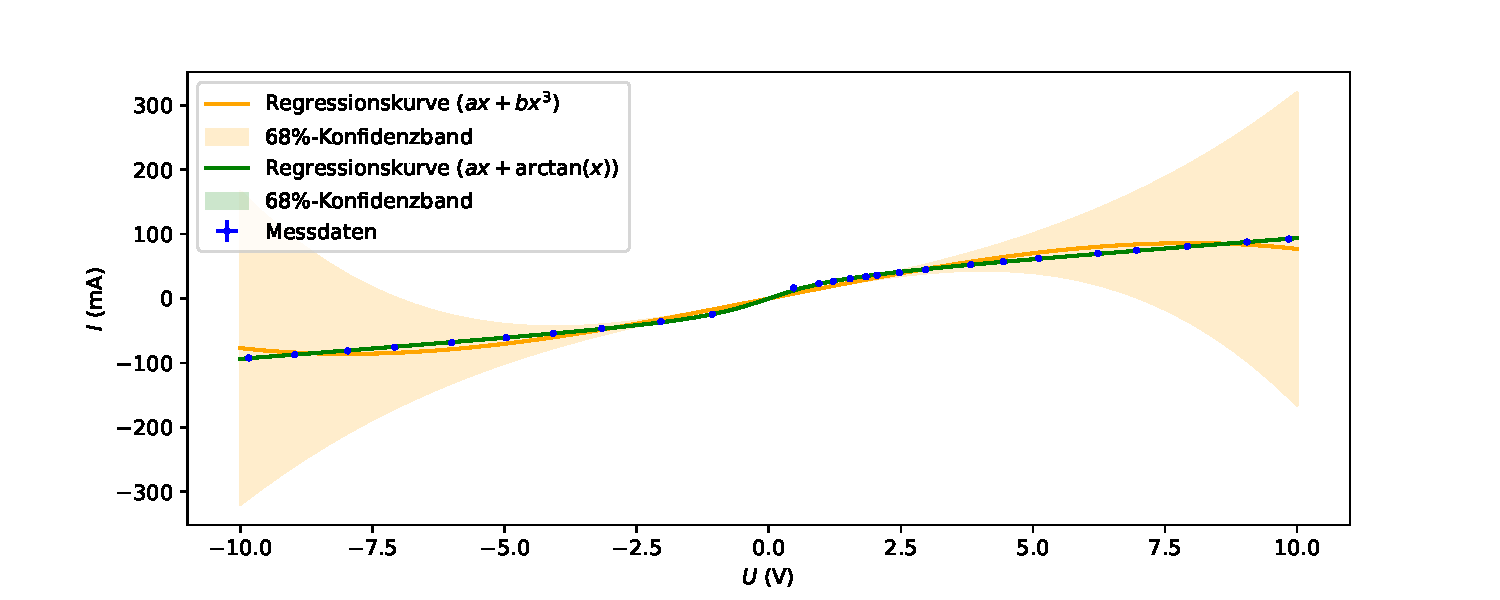
\includegraphics[width=\linewidth]{plot2}%
\vspace*{-1.28cm}\\ % ugly hack
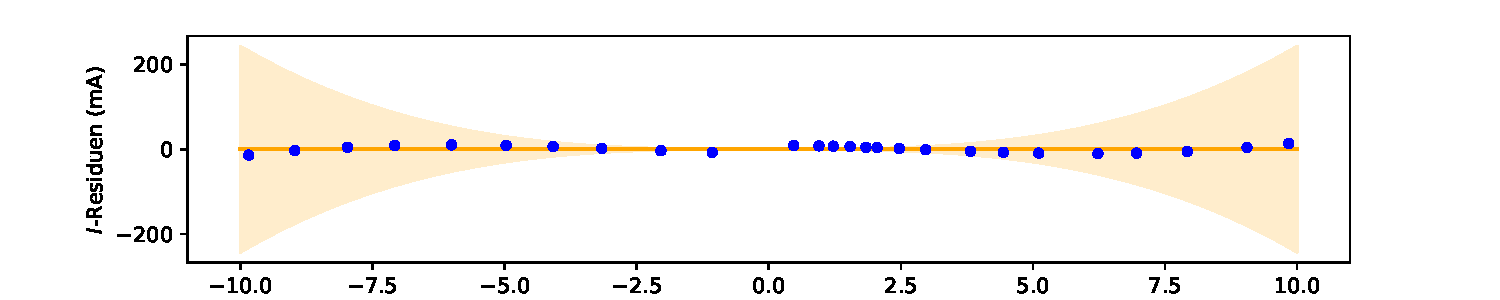
\includegraphics[width=\linewidth]{plot2residuen1}
\vspace*{-1.38cm}\\ % ugly hack
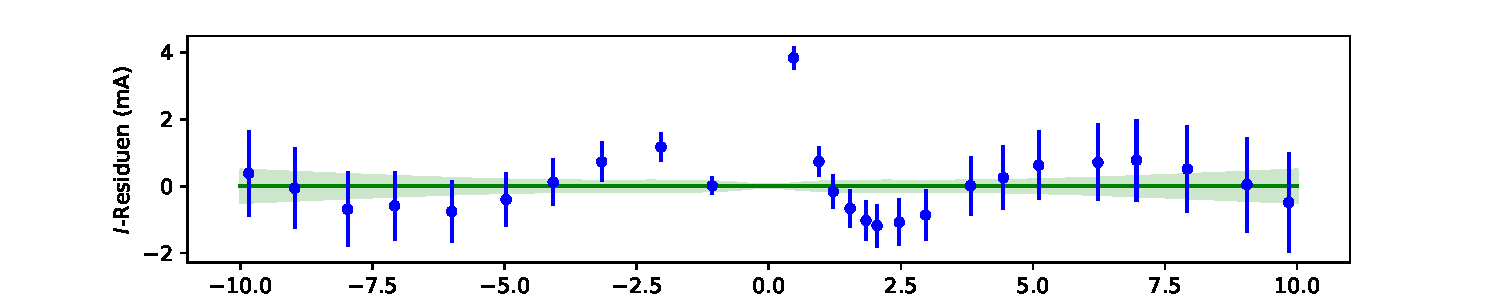
\includegraphics[width=\linewidth]{plot2residuen2}
\caption{Kennlinie der Glühlampe Residuendiagramm (unten)}\label{fig2}
\end{figure}

\begin{figure}
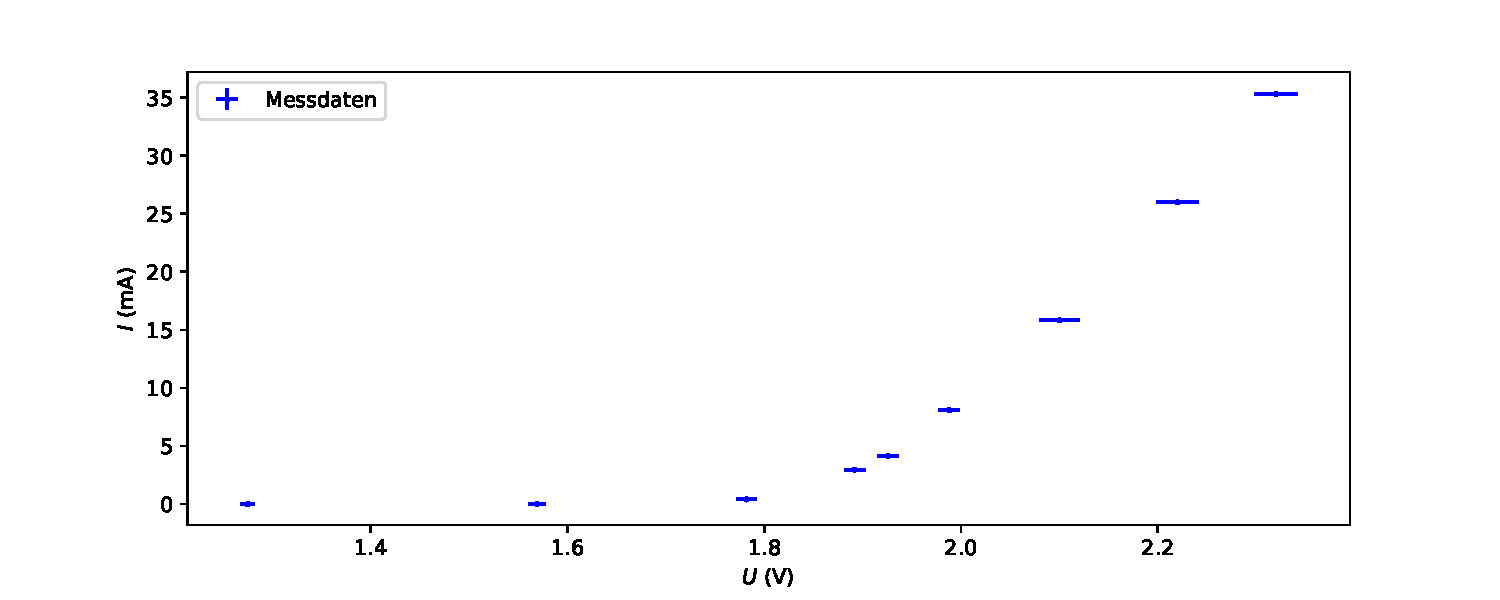
\includegraphics[width=\linewidth]{plot3}%
\caption{Kennlinie der LED}\label{fig3}
\end{figure}
\begin{figure}
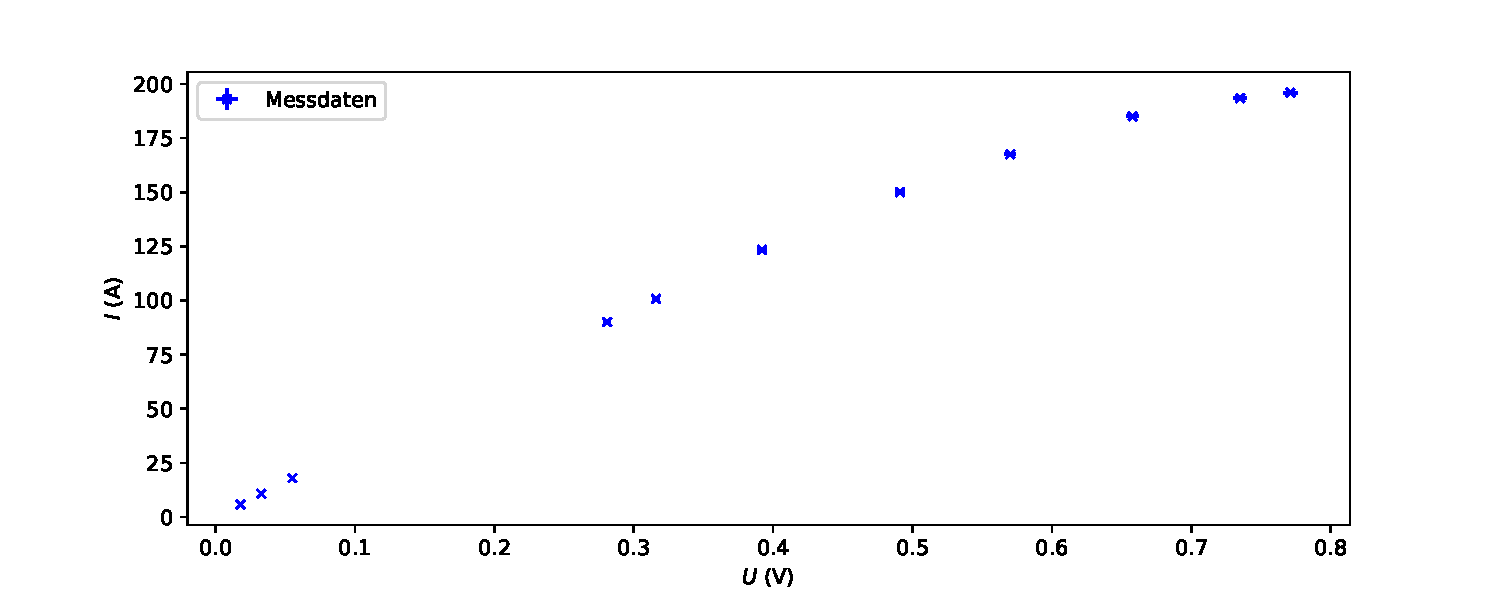
\includegraphics[width=\linewidth]{plot4}%

\caption{Kennlinie des unbekannten Bauteils}\label{fig4}
\end{figure}

\subsection{Widerstand der Glühlampe}

Bei \SI{0,47(12)}{\V} haben wir einen Widerstand von \SI{28,66(97)}{\ohm} erhalten. Mit kleineren Spannungen hätten wir sicherlich auch noch kleinere Widerstände erhalten. Die Regressionsgeraden ergeben hier keine sinnvollen Ergebnisse für den kleinsten Widerstand, da sie in diesem Bereich zu sehr von den tatsächlichen Messwerten abweichen.
Der höchste durch Messung bestimmte Widerstand beträgt \SI{106,7(18)}{\ohm}. Hier kann nur die arctan-Regressionsgerade sinnvolle Aussagen über den Widerstand bei noch größerer Helligkeit liefern. Bei maximaler Helligkeit wären das \SI{163.170(2)}{\ohm}.

\subsection{LED ohne Vorwiderstand}

Wir wollen berechnen, welcher Strom durch die LED geflossen wäre, wenn wir keinen Vorwiderstand verwendet hätten. Da wir leider nicht bedacht haben, die Gesamtspannung zu messen, werden wir diese aus dem Strom $I$ und dem angegebenen Vorwiderstand $R_{\rm{V}}$ berechnen. Der Strom durch die LED ohne Vorwiderstand berechnet sich dann folgendermaßen:
\[
I_{\rm{LED}} = \frac{U_{\rm{LED}}+I \cdot R_{\rm{V}}}{R_{\rm{LED}}}
\]
Wir erhalten ohne Widerstand eine deutlich steiler ansteigende Kennlinie (siehe \cref{fig5}).
\begin{figure}
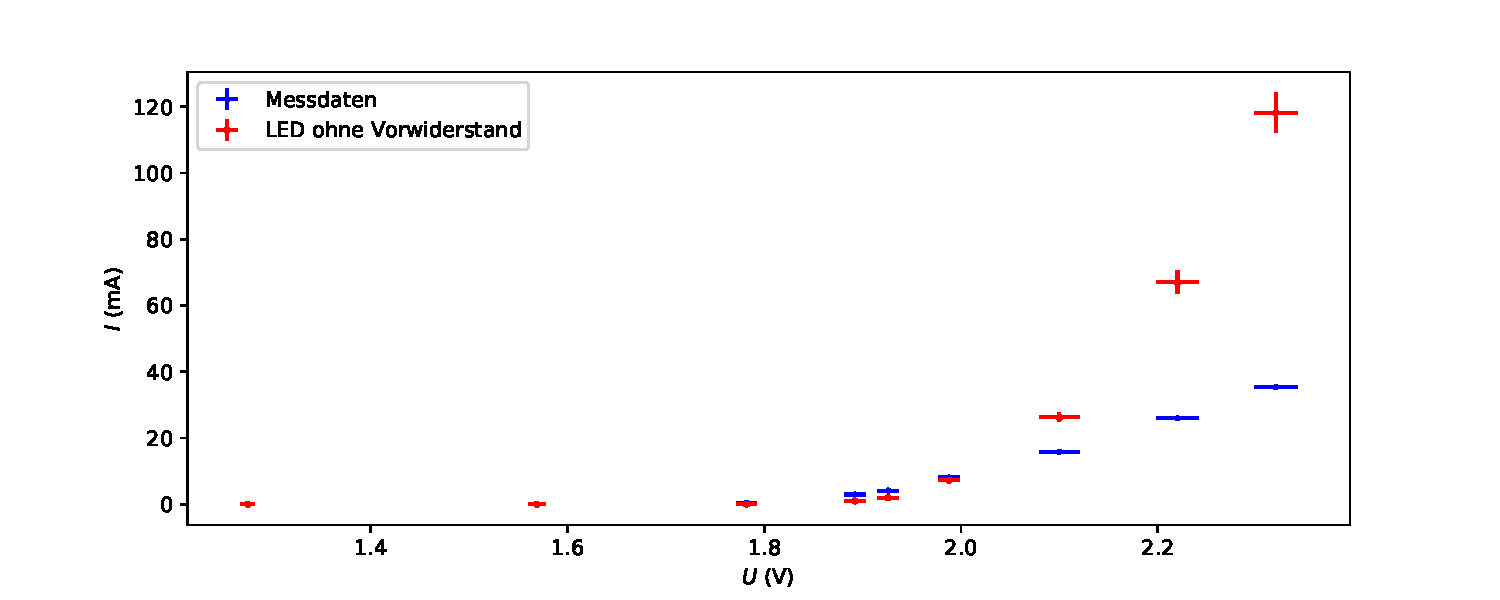
\includegraphics[width=\linewidth]{plot5}%

\caption{Kennlinie der LED ohne Vorwiderstand}\label{fig5}
\end{figure}
\subsection{Literaturvergleich}

Wir wollen den von uns gemessenen Widerstand mit dem Nominalwert $R_{\text{lit}} = \SIu{R1_lit}{dR1_lit}{\ohm}$ vergleichen.
Es bietet sich an das Inverse der Steigung der Regressionsgeraden $R = \SIu{R1}{dR1}{\ohm}$ dafür zu verwenden, da wir so eine gute Mittelung der Messwerte erhalten. Mit $t = \SIp{1}{t}$ stellen wir eine gute Verträglichkeit mit dem Literaturwert fest.

\section{Diskussion}



\subsection{unbekanntes Bauteil}

Beim Messen der Strom-Spannungs-Kennlinie des unbekannten Bauteils fiel uns besonders der lineare Verlauf der Kennlinie bei geringen Spannungen und die zeitliche Änderung der Spannung auf. Der Widerstand nahm mit der Zeit zu. Eine mögliche Erklärung wäre, dass das Bauteil ein PTC-Widerstand ist, der sich mit der Zeit aufgrund der eigenen Leistung erwärmt. Das würde erklären, wieso der Widerstand wieder abnahm, wenn man das Netzgerät ausschaltete. Ausschließen konnten wir den technischen Widerstand, da sich dieser zeitlich nicht so stark ändert. Die Diode konnten wir auch ausschließen, da der Widerstand in beide Richtungen gleich war,den Transistor, weil das Bauteil zweipolig war. Spule und den Kondensator konnten es auch nicht sein, weil keine Ladung gespeichert wurde, der Strom nicht wie es für einen Kondensator typisch wäre, bis auf 0A abgenommen hat und die Spannung gestiegen ist, anstatt wie bei einer Spule zu sinken.

\subsection{Verbesserung der Messung}

Die mit Abstand größten Messungenauigkeiten haben wir, wie bereits erwähnt, bei der LED, aufgrund einer schlechten Wahl der Schaltung, erhalten. Hier wäre es möglich gewesen, die Messgenauigkeit bei geringen Spannungen und Strömen mit der stromrichtigen Schaltung zu verbessern.
Bei der Glühlampe wäre es für die Bestimmung des Widerstands bei kleinen Spannungen hilfreich gewesen, wenn wir in diesem Bereich mehr Messergebnisse aufgenommen hätten.
Bei unserem unbekannten Bauteil hatten wir Spannungen, die sich zeitlich geändert haben. Es wäre noch interessant gewesen die Messergebnisse kurz nach dem Einschalten aufzunehmen, um zu schauen, ob wir dann auch für größere Spannung eine Gerade erhalten hätten.
\appendix


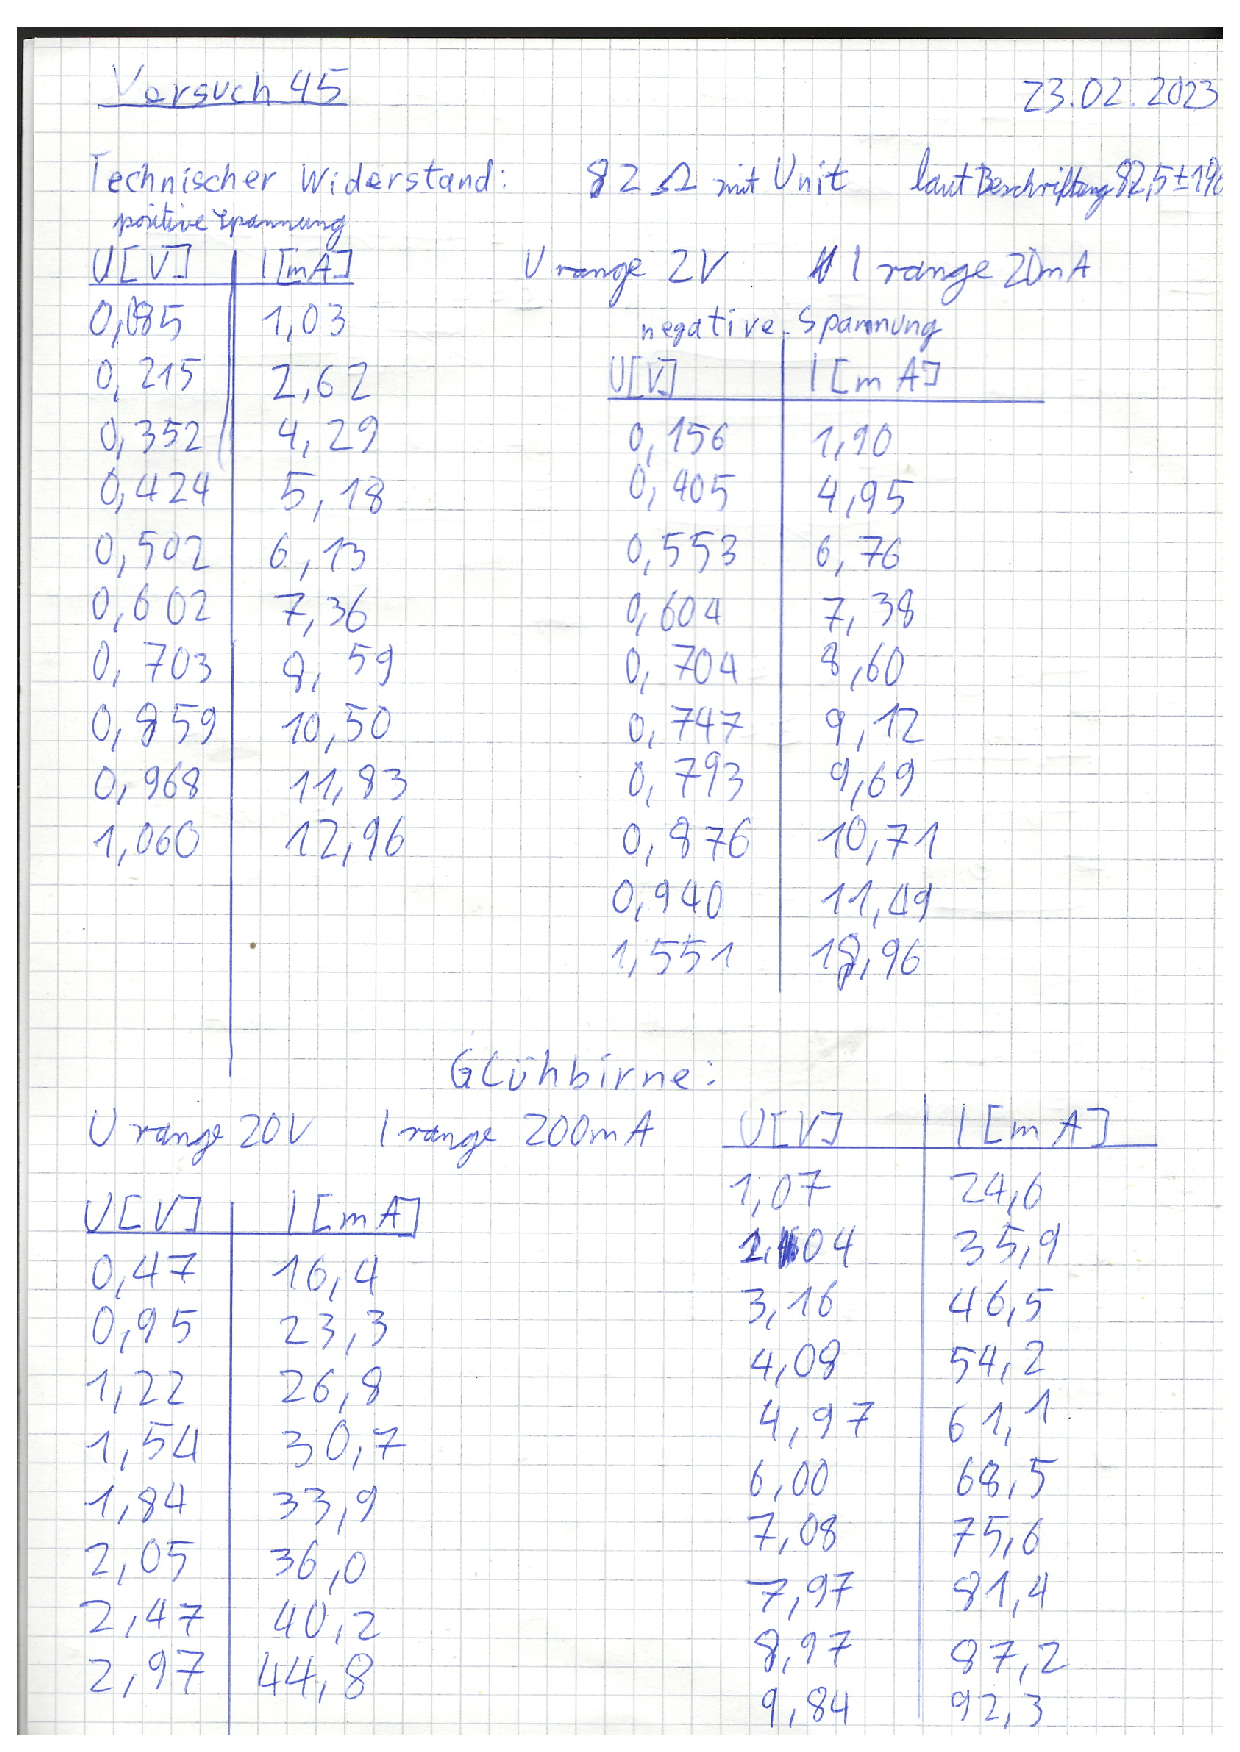
\includepdf[pages=1,scale=0.75,pagecommand={\section{Versuchsnotizen}}]{labnotes2.pdf}
\includepdf[pages=2-,scale=1,pagecommand={},linktodoc=true]{labnotes2.pdf}


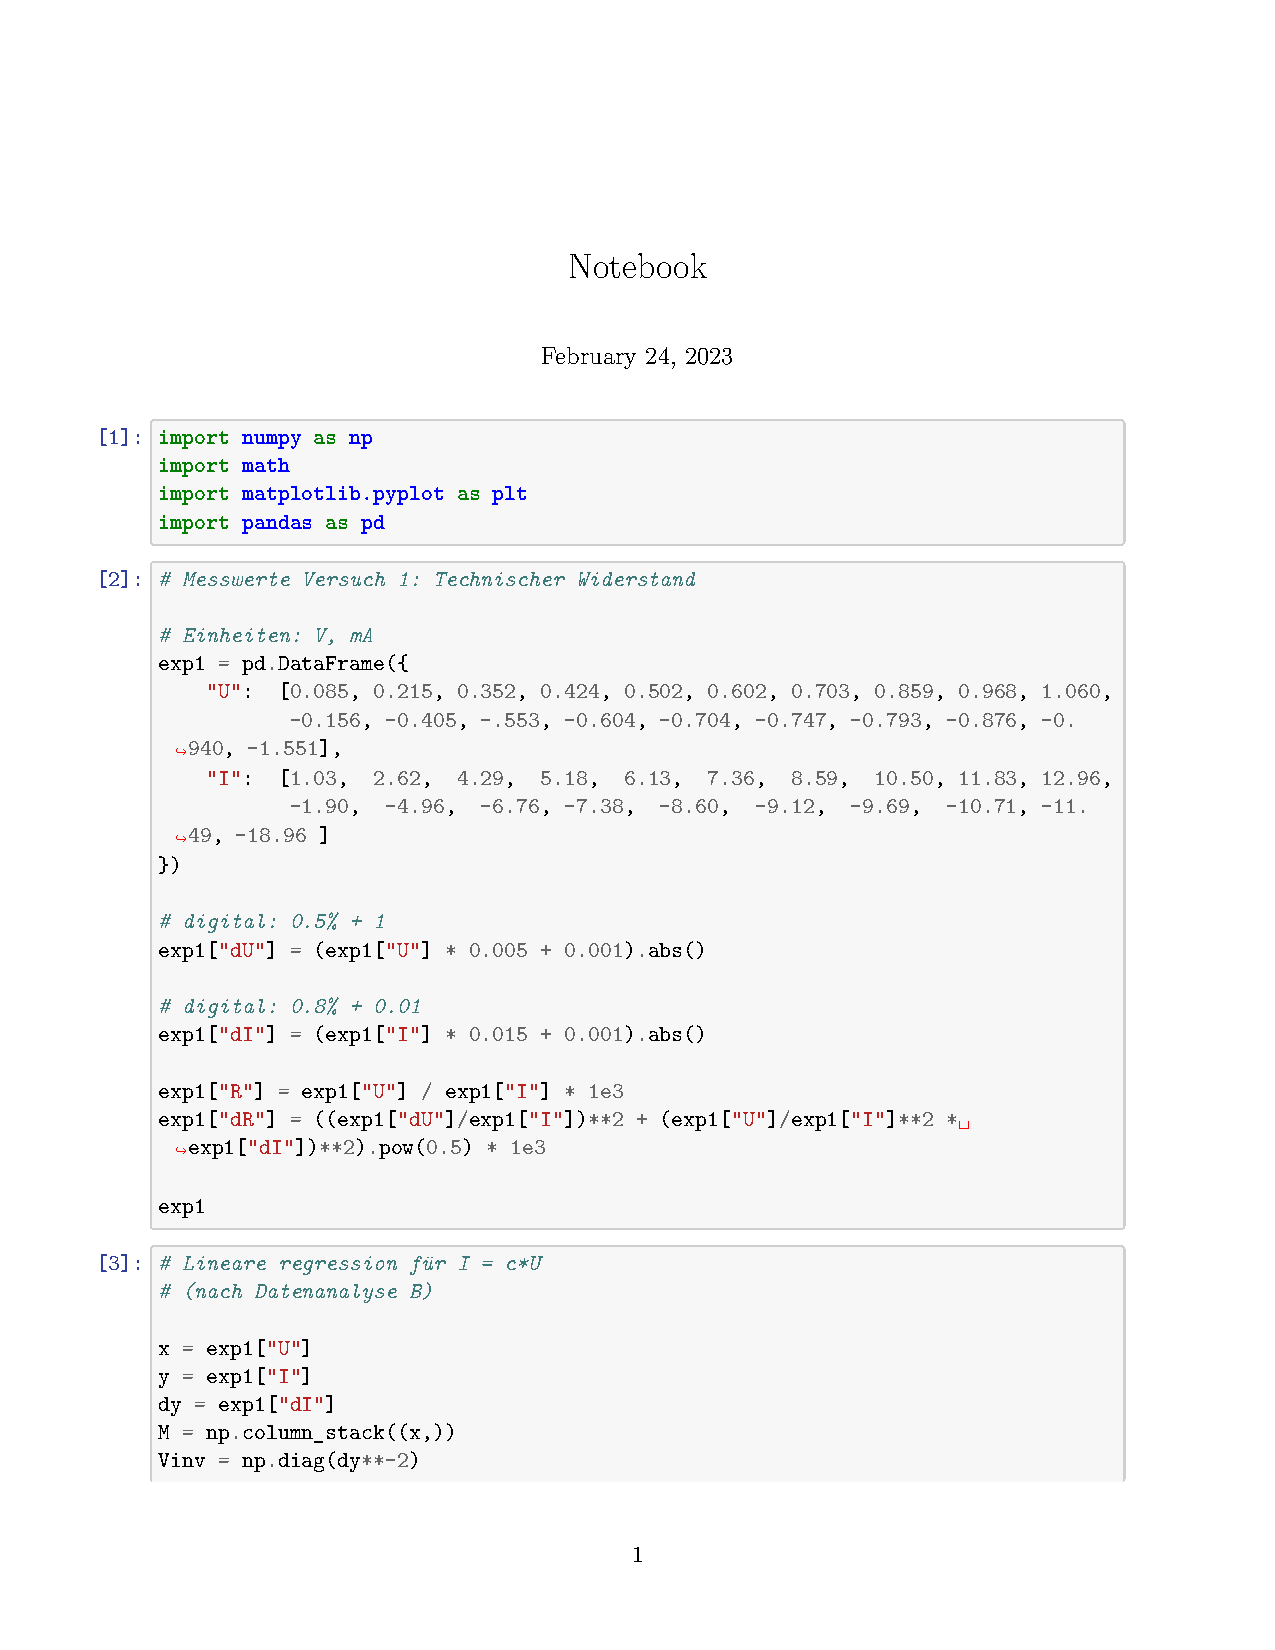
\includepdf[pages=1,scale=1,pagecommand={\section{Jupyter-Quellen}}]{Notebook.pdf}
\includepdf[pages=2-,scale=1,pagecommand={},linktodoc=true]{Notebook.pdf}

\end{document}
